\documentclass[a4paper,12pt]{article}
\usepackage[noabs,notoc]{HaotianReport}
\usepackage[numbered]{matlab-prettifier} % for matlab code

\title{第一次作业}
\author{刘昊天}
\authorinfo{电博181班, 2018310648}
\runninghead{高等电力网络分析}
\studytime{2018年11月}

\begin{document}
    \maketitle
    %\newpage
    \section{节点导纳矩阵的计算与分析}
    \subsection{题目1}
    \paragraph{题目描述} 请阅读参考程序1,理解并解读每一模块的功能与实现方法。试用自己的方法计算节点不定导纳矩阵Y0,并以地为参考节点生成导纳矩阵Y。
    \subsubsection{程序解读}
    \begin{enumerate}
      \item 导入MatPower的IEEE 9节点模型,并给出了模型信息。N为节点数量,b为支路数量。
      \begin{lstlisting}[style=Matlab-editor,basicstyle=\mlttfamily]
mpc = case9();
N = size(mpc.bus,1);
b = size(mpc.branch,1);
      \end{lstlisting}
      \item 生成不包含接地支路的导纳矩阵。\\
      首先生成节点支路关联矩阵A,使用稀疏矩阵进行存储。mpc结构体中的branch矩阵储存了网络支路的信息,每一行为一条支路,其中第一列与第二列分别存储了支路的首节点、尾节点。生成的方式,是在首节点(行号)与支路(列号)之间赋值1,在尾节点(行号)与支路(列号)之间赋值-1。\\
      其次生成支路导纳矩阵yb,方法是计算每一条支路的复导纳并将其放在矩阵的对角元上。branch矩阵的第三列、第四列分别为支路电阻、支路电感,导纳由\cref{eq:y}给出。\\
      \begin{equation}
        \label{eq:y}
        y_i = (R_i + j \cdot X_i)^{-1}, i\in[1, b]
      \end{equation}
      最后生成不包含接地支路的导纳矩阵Y。\\
      \begin{lstlisting}[style=Matlab-editor,basicstyle=\mlttfamily]
A = sparse(mpc.branch(:,1:2),[1:b,1:b]',[ones(b,1),-ones(b,1)]);
yb = spdiags(1./(mpc.branch(:,3)+1j*mpc.branch(:,4)),0,b,b);
Y = A*yb*A';
display(det(Y));
      \end{lstlisting}
      采用求取行列式的方式验证此时Y的奇异性,输出值为-2.0717e-05 + 1.3435e-05i。可见该值接近于0,Y矩阵此时是奇异的。这是由于没有接地支路,整个网络悬空,自然无法通过电流求取电压,符合物理意义。
      \item 补充接地支路,生成导纳矩阵Y。\\
      首先生成节点支路关联矩阵A,使用稀疏矩阵进行存储。由于为接地支路,因此节点与支路之间的关联元素均为1。构建A的目的,是为了从支路的对地导纳中等效出节点的接地导纳。
      其次使用A从支路上等效出节点的接地导纳,并生成节点接地导纳向量y0。每条线路使用$\pi$型等值电路,对地导纳等效在线路两侧,各1/2。同时每个节点有自身的对地导纳,储存在bus矩阵的第五列(电导)与第六列(电纳)中。
      最后,将接地导纳向量y0加到Y矩阵的对角元上,形成导纳矩阵Y。
      \begin{lstlisting}[style=Matlab-editor,basicstyle=\mlttfamily]
A = sparse(mpc.branch(:,1:2),[1:b,1:b]',ones(b,2));
y0 = A*1j*mpc.branch(:,5)/2 + mpc.bus(mpc.bus(:,1),5)+1j*mpc.bus(mpc.bus(:,1),6);
Y = Y + spdiags(y0,0,N,N);
      \end{lstlisting}
      \item 生成不定导纳矩阵Y0并测试奇异性
      \begin{lstlisting}[style=Matlab-editor,basicstyle=\mlttfamily]
Y0 = [Y,-y0;-y0.',sum(y0)];
display(det(Y0));
      \end{lstlisting}
      根据Y0的定义,将N+1节点定为大地节点,则可生成Y0阵。计算其行列式值,结果为6.7246e-06 + 8.5978e-06i。这表明Y0阵是奇异的,理由同样是没有参考节点。
    \end{enumerate}
    \subsubsection{不定导纳矩阵Y0生成}
    生成Y0矩阵时,不同于参考程序的思路,我们可以将大地节点作为N+1号节点,直接写出全网的节点支路关联矩阵,并计算全网的支路导纳。对于线路的对地导纳,我们可以用$\pi$形等值电路将导纳等效到节点上;对于节点的接地导纳,可以将其看做一条对地的支路。该思路生成Y0的程序如\cref{lst:q1p1}所示。
    \begin{lstlisting}[style=Matlab-editor,basicstyle=\mlttfamily,label=lst:q1p1,caption={不定节点导纳矩阵Y0生成程序}]
%% A0
nodeA = [mpc.branch(:,1);mpc.branch(:,2);(N+1)*ones(N,1);(1:N)'];
branchA = [1:b,1:b,b+(1:N),b+(1:N)]';
valueA = [ones(b,1);-ones(b,1);-ones(N,1);ones(N,1)];
A0 = sparse(nodeA, branchA, valueA);
%% yb
A = sparse(mpc.branch(:,1:2),[1:b,1:b]',ones(b,2));
y0 = A*1j*mpc.branch(:,5)/2 + mpc.bus(mpc.bus(:,1),5) + 1j*mpc.bus(mpc.bus(:,1),6);
yb = spdiags([1./(mpc.branch(:,3)+1j*mpc.branch(:,4));y0],0,b+N,b+N);
%% Y0 Y
Y0 = A0*yb*A0';
    \end{lstlisting}
    \subsubsection{导纳矩阵Y生成}
    由于大地节点是N+1号节点,因此直接截取Y0阵的前N行N列,即可得到导纳矩阵Y。
    \begin{lstlisting}[style=Matlab-editor,basicstyle=\mlttfamily]
Y = Y0(1:N, 1:N);
    \end{lstlisting}
    \subsection{题目2}
    \paragraph{题目描述} 调用matpower的makeYbus函数生成导纳矩阵Y,对比自己得到的Y,是否一致?请仔细阅读makeYbus函数及matpower手册,解释matpower生成Y矩阵的原理,注意其对移相器、变压器、接地支路的处理方法。发掘matpower在计算实现过程中涉及到的编程技巧。

    调用makeYbus函数计算得到Ybus矩阵,同自己生成的Y进行对比,程序及得到结果如下。该误差非常小,属于计算过程中由于步骤的不同,导致的浮点误差。因此自己得到的Y和makeYbus生成的导纳矩阵是一致的。
    \begin{lstlisting}[style=Matlab-editor,basicstyle=\mlttfamily]
%% makeYbus
disp('makeYbus');
[Ybus, ~, ~] = makeYbus(mpc);
disp(Ybus - Y);
% 输出:(9,9)      0.0000e+00 - 3.5527e-15i
    \end{lstlisting}

    makeYbus函数为了处理移相器支路,采用了不同的生成方式,MATPOWER的说明文档[TODO:cite]中对生成方式进行了说明。首先,将支路建立成一个二端口的形式,也就是变压器、移相器、输电线均被建立为一个通用支路模型,如\cref{fig:branch}所示。其中,$v_f,i_f$为首节点电压电流,$v_t,i_t$为尾节点电压电流,$N=\tau e^{j\theta_{shift}}$为变压器变比,包含了变压器档位和移相器相位,$y_s=\frac{1}{r_s+j x_s}$及$b_c$均为$\pi$形等值线路参数。由此我们可以得到该二端口网络的方程,如\cref{eq:branch}所示。

    \begin{figure}
      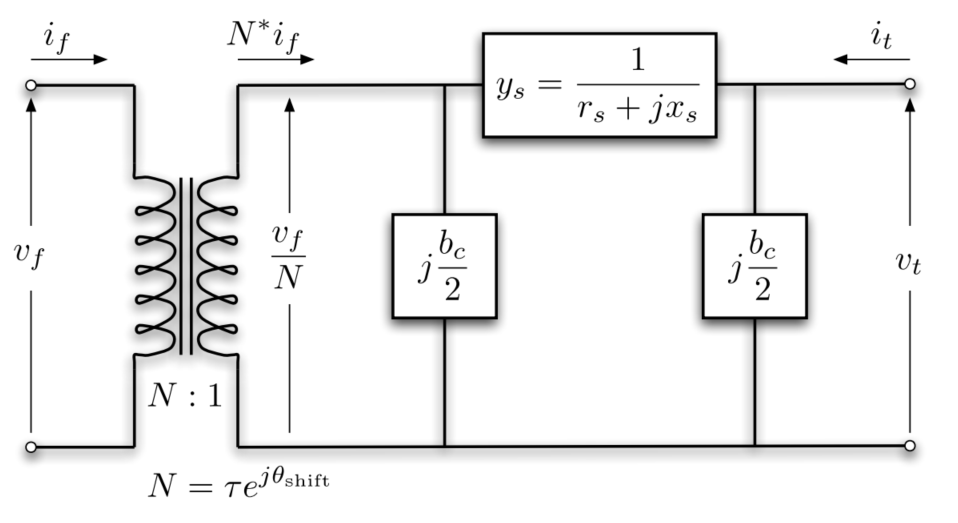
\includegraphics[width=0.95\linewidth]{branch}
      \caption{通用支路模型}
      \label{fig:branch}
    \end{figure}
    \begin{equation}
      \label{eq:branch}
      \begin{aligned}
        \begin{bmatrix}
          i_f\\
          i_t
        \end{bmatrix} &= Y_{br}
        \begin{bmatrix}
          v_f\\
          v_t
        \end{bmatrix} \\
        Y_{br} &= \begin{bmatrix}
          (y_s+j\frac{b_c}{2})\frac{1}{\tau^2} & -y_s\frac{1}{\tau e^{-j\theta_{shift}}} \\
          -y_s\frac{1}{\tau e^{j\theta_{shift}}} & y_s+j\frac{b_c}{2}
      \end{bmatrix}\\
      Y_{br}^i &=
      \begin{bmatrix}
        y_{ff}^i & y_{ft}^i\\
        y_{tf}^i & y_{tt}^i
      \end{bmatrix}
      \end{aligned}
    \end{equation}

    将网络中的节点按照支路的首尾分为首节点和尾节点,则我们可以构造向量$Y_{ff},Y_{ft},Y_{tf},Y_{tt}$描述网络。为了通过$Y_{br}^i$生成这些矩阵,引入支路节点关联矩阵$C_f, C_t$。该矩阵行号为支路,列号为节点,如果有关联则元素为1,否则为0。另外,各节点接地导纳可表示为$y_{sh}^i=g_{sh}^i+j b_{sh}^i$,$Y_{sh}=G_sh+jB_{sh}$为接地导纳向量。

    网络方程表示为\cref{eq:net},其中导纳矩阵表示为\cref{eq:ybus}。这就是MATPOWER对网络矩阵的处理方式。
    \begin{equation}
      \label{eq:net}
      \begin{aligned}
        I_f &= Y_f V \\
        I_t &= Y_t V
      \end{aligned}
    \end{equation}
    \begin{equation}
      \label{eq:ybus}
      \begin{aligned}
          Y_f = diag(Y_{ff})C_f+diag(Y_{ft})C_t\\
          Y_t = diag(Y_{tf})C_f+diag(Y_{tt})C_t\\
          Y_{bus} = C_f^TY_f+C_t^TY_t+diag(Y_{sh})
      \end{aligned}
    \end{equation}

    TODO:编程技巧
    \subsection{题目3}
    \paragraph{题目描述} 探讨Y矩阵的各类特性(包括但不限于:稀疏性、对角占优、非奇异性等),并用计算结果进行验证。

    编写验证程序如\cref{lst:q1q3p1}所示,结果如\cref{lst:q1q3p2,fig:diagpri}示。

    可见,对于稀疏性而言,计算矩阵的稀疏度(非零元素数量占比)结果为0.3333,这表明矩阵只有33.33\%的元素是非零的,因此是稀疏的。对于对角占优性而言,\cref{fig:diagpri}描述了矩阵每行对角元绝对值和每行除去对角元外的最大绝对值元素绝对值的比值分布。可以看到,对于IEEE-9节点网络和IEEE-118节点网络来说,大部分的比值都分布在1的右侧,这表明绝大多数行都是对角占优的。特别对于IEEE-9节点网络来说,所有行都可以认为是对角占优的。对于非奇异性而言,计算矩阵的行列式,得到2.443e+09,远大于0,说明矩阵时非奇异的。

    \begin{lstlisting}[style=Matlab-editor,basicstyle=\mlttfamily,label=lst:q1q3p1,caption={矩阵特性验证程序}]
%% feature of Y
disp('sparse');
fprintf('sparse degree = %.3f\n', nnz(Y)/numel(Y));
disp('diagonal priority');
f=figure();
yyaxis left;
histDiagPri(mpc);
ylabel('num');
yyaxis right;
histDiagPri(case118());
xlabel('diagElem / max(abs(otherColumnElem))');
ylabel('num');
legend('case9','','case118','');
saveas(f, [pwd '\meta\diagpri.png']);
close(f);
disp('non-singularity');
fprintf('|det(Y)| = %s\n', abs(det(Y)));
    \end{lstlisting}
    \begin{lstlisting}[label=lst:q1q3p2,caption={矩阵特性验证结果}]
sparse
sparse degree = 0.333
diagonal priority
non-singularity
|det(Y)| = 2.443121e+09
    \end{lstlisting}
    \begin{figure}
      \includegraphics[width=0.95\linewidth]{../meta/diagpri.png}
      \caption{Y阵对角占优特性研究}
      \label{fig:diagpri}
    \end{figure}
    \subsection{题目4}
    \paragraph{题目描述} 实现对Y矩阵的因子表分解(分步进行,明确操作流程与原理)

    使用课堂上讲解的分解算法,LU分解及LDU分解程序见附录中的\cref{lst:calcLU,lst:calcLDU}。通过验证程序计算分解后与原矩阵偏差的二阶矩,可以验证分解结果的正确性,如\cref{lst:q1q4p1}所示。可见,分解误差非常接近于0,所实现的因子表分解算法是正确的。
    \begin{lstlisting}[style=Matlab-editor,basicstyle=\mlttfamily,label=lst:q1q4p1,caption={因子表分解及正确性验证}]
%% LDU
disp('LDU');
[L, U] = calcLU(Y);
fprintf('LU error = %s\n', norm(full(L*U - Y)));
% 输出:LU error = 3.828143e-15
[L, D, U] = calcLDU(Y);
fprintf('LDU error = %s\n', norm(full(L*D*U - Y)));
% 输出:LDU error = 1.917847e-15
    \end{lstlisting}
    \section{网络方程修正解法}
    已知Y、Z为case9标准系统的导纳、阻抗矩阵,已知Y的LDU分解。现在case9系统的7、9节点间添加一条支路,参数见r、x、b分别为0.0213、0.108、0.239(标幺值)。
    \subsection{题目1}
    \paragraph{题目描述} 阅读参考程序2,理解并解读每一模块的功能与实现方法。试用自己的方法求新系统的导纳、阻抗矩阵。
    \subsubsection{程序解读}
    \begin{enumerate}
      \item 导入新模型并给出相关变量。其中inn、jnn分别为新支路的首尾节点编号。
      \begin{lstlisting}[style=Matlab-editor,basicstyle=\mlttfamily]
%% previous
expY();
Zi = inv(Y);
%% Import case
mpc_m = case9_modified();
inn = mpc_m.branch(end,1);
jnn = mpc_m.branch(end,2);
      \end{lstlisting}
      \item 修正导纳矩阵。\\
      首先计算新增支路的导纳,以及支路两端等效的接地导纳。然后构造新支路的关联矢量,并将修正块加到原矩阵上。最后将接地导纳加到原矩阵的对角元上,完成修正。
      \begin{lstlisting}[style=Matlab-editor,basicstyle=\mlttfamily]
%% Modify Y
yl = 1./(mpc_m.branch(end,3)+1j*mpc_m.branch(end,4));
bl = mpc_m.branch(end,5)/2;
Ml = sparse([inn,jnn],1,[1,-1],N,1);
Ym = Y + Ml*yl*Ml' + sparse([inn,jnn],[inn,jnn],[1j;1j]*bl,N,N);
      \end{lstlisting}
      \item 修正阻抗矩阵。\\
      利用矩阵求逆辅助定理,对增加线路的线路导纳及等效出的对地支路进行修正。每次修正中,分别构造关联矢量和修正量,依次修正即可。
      \begin{equation}
        \begin{aligned}
          Y &= Y_0+M_\alpha y_\alpha M_\alpha^T\\
          Z=Y^{-1}&= Z_0 -Z_0 M_\alpha \widetilde z_{\alpha\alpha} M_\alpha^T Z_0\\
          \widetilde z_{\alpha\alpha}&=y_\alpha^{-1}+M_\alpha^T Z_0 M_\alpha
        \end{aligned}
      \end{equation}
      \begin{lstlisting}[style=Matlab-editor,basicstyle=\mlttfamily]
%% Modify Z
% Add line reactance
zl = 1/yl + Ml'*Zi*Ml;
Zm = Zi - Zi*Ml/zl*Ml'*Zi;
% Add shunt reactance at initial
zl = -1j/bl + Zm(inn,inn);
Zm = Zm - Zm(:,inn)/zl*Zm(inn,:);
% Add shunt reactance at end
zl = -1j/bl + Zm(jnn,jnn);
Zm = Zm - Zm(:,jnn)/zl*Zm(jnn,:);
      \end{lstlisting}
    \end{enumerate}
    \subsubsection{导纳矩阵修正}
    该修正方法和参考程序类似。区别在于使用了一种编程技巧,即读取了MATPOWER的标号函数,将原来的常数下标换成了F\_BUS、T\_BUS这样的变量,使得程序易读。TODO
    \begin{lstlisting}[style=Matlab-editor,basicstyle=\mlttfamily,label=lst:q2q1p1,caption={导纳矩阵修正程序}]
    \end{lstlisting}
    \subsubsection{阻抗矩阵修正}
    TODO。本报告所采用的的
    \begin{lstlisting}[style=Matlab-editor,basicstyle=\mlttfamily,label=lst:q2q1p2,caption={阻抗矩阵修正程序}]
    \end{lstlisting}
    \subsection{题目2}
    \paragraph{题目描述} 讨论并验证在已添加支路的系统中去除该支路的LDU修正方法与结果。请思考:需要做几次修正?因子表的秩1因子修正与局部再分解的计算效率如何?修正法的应用场景与意义?

    去除该支路的方法是添加一条负支路,其线路导纳与对地导纳和原支路符号相反,其他参数与原支路相同。这种情形下,可以采用秩1因子修正法或局部再分解法。

    \subsubsection{秩1因子修正法}
    对于一个一般的矩阵,其秩1因子分解的修正可表示为
    \begin{equation}
      \label{eq:r1eq}
      \widetilde A = A + \Delta A = A + MaN^T = LDU + MaN^T = \widetilde L \widetilde D \widetilde U
    \end{equation}
    其中a为标量。

    先考虑矩阵的第一行第一列。将$L,D,U$首行首列的元素分块写出,并将$M,N$的首行元素也分块写出
    \begin{equation}
      \widetilde L = \begin{bmatrix}
        1 & \\
        \widetilde l_1 & \widetilde L_1
      \end{bmatrix}, \widetilde D = \begin{bmatrix}
        \widetilde d_1 & \\
         & \widetilde D_1
      \end{bmatrix}, \widetilde U = \begin{bmatrix}
        1 & \widetilde u_1\\
         & \widetilde U_1
      \end{bmatrix}, M = \begin{bmatrix}
        m_1 \\ M_1
      \end{bmatrix}, N = \begin{bmatrix}
        n_1 \\ N_1
      \end{bmatrix}
    \end{equation}

    将矩阵的分块形式带入\cref{eq:r1eq},可以得到方程
    \begin{equation}
      \label{eq:r1meq}
      \begin{aligned}
        \widetilde L \widetilde D \widetilde U &= LDU + MaN^T\\
        \begin{bmatrix}
          \widetilde d_1 & \widetilde d_1 \widetilde u_1 \\
          \widetilde l_1 \widetilde d_1 & \widetilde l_1 \widetilde d_1 \widetilde u_1 + \widetilde L_1 \widetilde D_1 \widetilde U_1
        \end{bmatrix}& = \begin{bmatrix}
          d_1 & d_1 u_1\\
          l_1 d_1 & l_1 d_1 u_1 + L_1 D_1 U_1
        \end{bmatrix} + \begin{bmatrix}
          m_1an_1&m_1aN_1^T\\
          M_1an_1&M_1aN_1^T
        \end{bmatrix}
      \end{aligned}
    \end{equation}

    \cref{eq:r1meq}中有四个分块方程,使用左上、右上、左下三个方程可以求得$\widetilde l_1, \widetilde d_1, \widetilde u_1$的表达式
    \begin{equation}
      \begin{aligned}
        \widetilde d_1 &= d_1 +m_1an_1\\
        \widetilde l_1 &= l_1+\widetilde M_1 a n_1 \widetilde d_1^{-1}\\
        \widetilde u_1 &= u_1+\widetilde d_1^{-1}m_1a\widetilde N_1^T
      \end{aligned}
    \end{equation}
    其中$\widetilde M_1=M_1-l_1m_1, \widetilde N_1^T=N_1^T-n_1u_1$。

    对于右下角的方程,可以化为新问题
    \begin{equation}
      \left\{
        \begin{array}{l}
          \widetilde A_1 = \widetilde L_1 \widetilde D_1 \widetilde U_1 = A_1 + \Delta A_1 \\
          A_1 = L_1 D_1 U_1\\
          \Delta A_1 = l_1d_1u_1-\widetilde l_1 \widetilde d_1 \widetilde u_1 + M_1aN_1^T
        \end{array}
      \right.
    \end{equation}
    化简$\Delta A_1$可得
    \begin{equation}
      \Delta A_1=\widetilde M_1 \widetilde a \widetilde N_1^T
    \end{equation}
    其中
    \begin{equation}
      \widetilde a=a-an_1\widetilde d_1^{-1}m_1a
    \end{equation}

    根据以上原理,设计迭代算法,同课件上给出的一致。特别地,此处问题为对称修正,可以认为$M=N, L=U^T$,利用该条件可以化简算法,实现程序见\cref{lst:modifyLDUr1_org}。进一步使用稀疏矢量技术,算法效率得到提升,实现程序见\cref{lst:modifyLDUr1}。另外,\cref{lst:generateSm}中实现了道路集的获取,这是稀疏矢量技术所需要的。

    在本例中,应用秩1因子修正法的程序如\cref{lst:q2q2r1}所示。去除该支路分三步进行,分别去除支路导纳、首节点接地导纳、尾节点接地导纳。为了验证修正的正确性,将其与直接去除支路得到的Y阵进行比较,并计算误差的二阶矩。结果显示,误差很小,证明本方法正确。
    \begin{lstlisting}[style=Matlab-editor,basicstyle=\mlttfamily,caption={秩1因子修正法去除支路},label=lst:q2q2r1]
[L, D, U] = calcLDU(mpYm);
[Lm1, Dm1, Um1] = modifyLDUr1(D, U, Ml, -ybr);
[Lm1, Dm1, Um1] = modifyLDUr1(Dm1, Um1, sparse(fbn, 1, 1, N, 1), -1j * bbn);
[Lm1, Dm1, Um1] = modifyLDUr1(Dm1, Um1, sparse(tbn, 1, 1, N, 1), -1j * bbn);
disp('modify LDU - Rank 1');
fprintf('ldu-r1 error = %s\n', norm(full(Y - Lm1*Dm1*Um1)));
% 输出:ldu-r1 error = 6.776442e-15
    \end{lstlisting}
    \subsubsection{局部再分解法}
    如果被修正部分集中在矩阵的右下角,则可以推导因子表的局部再分解方法。如果分布在矩阵当中,则根据受影响的范围(可证明为道路集)将该子矩阵视为右下角,从而修正矩阵。因此,可以首先假设修正是集中在右下角的。

    将原网络矩阵因子分解写成分块形式
    \begin{equation}
      \begin{aligned}
        A=\begin{bmatrix}
          A_{11}&A_{12}\\A_{21}&A_{22}
      \end{bmatrix}&=\begin{bmatrix}
        L_{11}&0\\L_{21}&L_{22}
      \end{bmatrix} \begin{bmatrix}
        D_{11}&0\\0&D_{22}
      \end{bmatrix} \begin{bmatrix}
        U_{11}&U_{12}\\0&U_{22}
      \end{bmatrix} \\
      &=\begin{bmatrix}
        L_{11}D_{11}U_{11} & L_{11}D_{11}U_{11}\\
        L_{21}D_{11}U_{11} & L_{21}D_{11}U_{12} + L_{22}D_{22}U_{22}
    \end{bmatrix}
      \end{aligned}
    \end{equation}
    修正矩阵可写成分块形式
    \begin{equation}
      \begin{aligned}
        \widetilde A&=A+\Delta A=\begin{bmatrix}
        A_{11} & A_{12}\\ A_{21} & \widetilde A_{22}
      \end{bmatrix} \\
      \widetilde A_{22} = A_{22} + \Delta A_{22}
      \end{aligned}
    \end{equation}
    因子再分解过程也可以写成分块形式,下式可以通过矩阵乘法验证
    \begin{equation}
      \begin{aligned}
        \widetilde A &= \begin{bmatrix}
          A_{11}&A_{12}\\A_{21}&\widetilde A_{22}
        \end{bmatrix}=\begin{bmatrix}
          L_{11}&0\\L_{21}&\widetilde L_{22}
        \end{bmatrix} \begin{bmatrix}
          D_{11}&0\\0&\widetilde D_{22}
        \end{bmatrix} \begin{bmatrix}
          U_{11}&U_{12}\\0&\widetilde U_{22}
        \end{bmatrix} \\
      &=\begin{bmatrix}
        L_{11}D_{11}U_{11} & L_{11}D_{11}U_{11}\\
        L_{21}D_{11}U_{11} & L_{21}D_{11}U_{12} + \widetilde L_{22}\widetilde D_{22}\widetilde U_{22}
      \end{bmatrix} \\
        \widetilde A_{22} &= L_{21}D_{11}U_{12} + \widetilde L_{22}\widetilde D_{22}\widetilde U_{22}
      \end{aligned}
    \end{equation}
    变换形式可得
    \begin{equation}
      \widetilde A_{22}-A_{22}=\widetilde L_{22}\widetilde D_{22}\widetilde U_{22}-L_{22}D_{22}U_{22}=\Delta A_{22}
    \end{equation}
    令
    \begin{equation}
      \begin{aligned}
        \widetilde A_{22}'&=\widetilde L_{22}\widetilde D_{22}\widetilde U_{22}\\
        A_{22}'&=L_{22}D_{22}U_{22}
      \end{aligned}
    \end{equation}
    则有
    \begin{equation}
      \widetilde A_{22}'=A_{22}'+\Delta A_{22}
    \end{equation}
    由此可见,每次修正只需要求出$A_{22}'$,并将其修正,最后再分解即可。

    局部再分解法的实现程序见\cref{lst:modifyLDUlr},\cref{lst:generateSm}给出了道路集的求解方法。

    在本例中,修正的方式是首先导出一个$3\times 3$的矩阵修正块,代表对支路导纳及支路两端接地导纳的去除,随后将该修正块利用局部再分解法进行修正。为了验证修正的正确性,将其与直接去除支路得到的Y阵进行比较,并计算误差的二阶矩。修正程序及输出结果如\cref{lst:q2q2lr}所示。结果显示,误差很小,证明本方法正确。
    \begin{lstlisting}[style=Matlab-editor,basicstyle=\mlttfamily,label=lst:q2q2lr,caption={秩1因子修正法去除支路}]
%% Modify LDU - Local Re
dY = sparse([fbn, tbn], [fbn, tbn], [-1j * bbn, -1j * bbn], N, N);
dY = dY + Ml * -ybr * Ml.';
[Lm2, Dm2, Um2] = modifyLDUlr(D, U, dY);
disp('modify LDU - Local Re');
fprintf('ldu-lr error = %s\n', norm(full(Y - Lm2*Dm2*Um2)));
% 输出:ldu-lr error = 1.046696e-14
    \end{lstlisting}
    \subsubsection{方法比较}
    TODO
    \subsubsection{应用场景与意义}
    在修正范围小,受影响的节点少的情况下,TODO

    \subsection{题目3}
    \paragraph{题目描述} 探讨并用运算结果说明补偿法的物理意义(可以考虑使用“补偿电流”的方法)。
    \subsubsection{补偿电流法推导}
    为了解释补偿电流法的物理意义,本节对补偿电流法进行推导,以展示该方法的过程。首先应明确补偿法应用的场合,即物理背景。补偿法特别适用于注入电流不变,而又要对网络中不同部分发生局部变化时求网络方程的解(电压)的应用场合。这时通过矩阵求逆辅助定理,可以将网络的修正等效到电压或电流或前代回代计算中间量的变化上。这样只需要利用原来的导纳矩阵的因子表进行前代回代求解,省去了重新分解因子表的计算量。

    在电流不变的假设下,有
    \begin{equation}
      \begin{aligned}
        YV&=I\\
        (Y+\Delta Y)\widetilde V&=I\\
        \Delta Y&=M\delta y M^T
      \end{aligned}
    \end{equation}
    使用矩阵求逆辅助定理,有
    \begin{equation}
      \begin{aligned}
        \widetilde V&=(Y^{-1}-Y^{-1}McM^TY^{-1})I\\
        c&=(\delta y^{-1}+M^TY^{-1}M)^{-1}
      \end{aligned}
    \end{equation}
    使用补偿电流法,可以推导出补偿电流为
    \begin{equation}
      \begin{aligned}
        \Delta I&=-McM^TY^{-1}I\\
        \widetilde V&=Y^{-1}(I+\Delta I)
      \end{aligned}
    \end{equation}

    为了验证补偿电流法的正确性,编写程序及输出结果如\cref{lst:q2q3p1}所示,结果表明误差很小,本方法正确。
    \begin{lstlisting}[style=Matlab-editor,basicstyle=\mlttfamily,label=lst:q2q3p1,caption={补偿电流法}]
%% Compensation method
% Compensation current
V = sparse(1:N, 1, 1, N, 1);
I = Y * V;
deltay = sparse(1:3, 1:3, -[ybr, 1j * bbn, 1j * bbn], 3, 3);
M = sparse([fbn, tbn, fbn, tbn], [1,1,2,3], [1,-1,1,1], N, 3);
c = inv(inv(deltay) + M.' * inv(Y) * M);
deltaI = - M * c * M.' * inv(Y) * I;
Is = I + deltaI;
Vs = Y \ Is;
Vsorg = mpYm \ I;
disp('Compensation current');
fprintf('v error = %s\n', norm(full(Vsorg - Vs)));
% 输出:TODO
    \end{lstlisting}
    \subsubsection{补偿电流法物理意义}
    对于去掉一条支路的情况,可以等效为在一个端口($i,j,i<j$)上并联一条负阻抗支路$\delta y_l=-y_l$,同样等效为在端口注入一对符号相反的电流,$i$节点注入$-I_{ij}$,$j$节点注入$I_{ij}$,$I_{ij}$为原网络上并联$\delta y_l$后该支路上的电流。本例中$i=7,j=9$。

    为了求解$I_{79}$,可以从(7,9)端口看入做戴维南等效。戴维南等效电动势为端口开路电压,
    $$\dot E_{79}=M^T \dot V=TODO$$
    戴维南等效阻抗为
    $$Z_T=M^TY^{-1}M=TODO$$
    并联$\delta y_l$后,回路阻抗为
    $$c^{-1}=\delta y_l^{-1}+Z_T=TODO$$
    由此计算回路电流为
    $$\dot I_{ij}=\dot E_{ij}/c^{-1}=cM^TY^{-1}\dot I=TODO$$
    转换为向量形式的注入电流
    $$\Delta \dot I=-M\dot I_{ij}=-McM^TY^{-1}\dot I=TODO$$
    补偿后的注入电流为
    $$\widetilde {\dot I} = \dot I + \Delta \dot I=TODO$$
    最终求解得到变化后的网络解(电压)为
    $$\widetilde {\dot V} = Y^{-1} \widetilde {\dot I} = TODO$$
    \newpage
    \bibliography{report}
    \bibliographystyle{unsrt}
    \appendix
    \section{程序清单}
      \lstinputlisting[style=Matlab-editor,basicstyle=\mlttfamily,label=lst:hwtask,caption={全部作业任务}]{../hwtask.m}
      \lstinputlisting[style=Matlab-editor,basicstyle=\mlttfamily,label=lst:calcLU,caption={LU分解}]{../calcLU.m}
      \lstinputlisting[style=Matlab-editor,basicstyle=\mlttfamily,label=lst:calcLDU,caption={LDU分解}]{../calcLDU.m}
      \lstinputlisting[style=Matlab-editor,basicstyle=\mlttfamily,label=lst:generateSm,caption={生成道路集}]{../generateSm.m}
      \lstinputlisting[style=Matlab-editor,basicstyle=\mlttfamily,label=lst:modifyLDUr1_org,caption={秩1因子法因子修正}]{../modifyLDUr1_org.m}
      \lstinputlisting[style=Matlab-editor,basicstyle=\mlttfamily,label=lst:modifyLDUr1,caption={秩1因子法因子修正(稀疏向量)}]{../modifyLDUr1.m}
      \lstinputlisting[style=Matlab-editor,basicstyle=\mlttfamily,label=lst:modifyLDUlr,caption={局部再分解法因子修正}]{../modifyLDUlr.m}
      \lstinputlisting[style=Matlab-editor,basicstyle=\mlttfamily,label=lst:histDiagPri,caption={观察主对角占优}]{../histDiagPri.m}
    \label{applastpage}
\iffalse
\begin{itemize}[noitemsep,topsep=0pt]
%no white space
\end{itemize}
\begin{enumerate}[label=\Roman{*}.,noitemsep,topsep=0pt]
%use upper case roman
\end{enumerate}
\begin{multicols}{2}
%two columns
\end{multicols}
\fi
\end{document}
